\chapter{Introdução}

A computação ubíqua caracteriza-se pela existência de ambientes com inteligência computacional, \emph{smart spaces}, que por meio de diversos dispositivos, auxiliam um usuário na realização de uma tarefa. O termo ubíquo é devido ao fato da computação estar em todos os lugares, muitas vezes se apresentando de forma tão amigável que não notamos sua presença, e por esse motivo, a Computação Ubíqua também é chamada de Computação Invisível~\cite{gomes2007, weiser1993, weiser1999}. Dessa forma, os dispositivos trabalham harmonicamente a fim de evitar, sempre que possível, toda e qualquer intervenção humana. Faz-se necessário, inclusive, que tais sistemas sejam pró-ativos ~\cite{gomes2007, buzeto2010} e consigam determinar, com a ajuda de informações de contexto previamente coletadas, quais as melhores decisões a serem tomadas em determinados instantes. Deve-se considerar, ainda, a mobilidade ~\cite{gomes2007, buzeto2010, weiser1999} dos aparelhos presentes e regidos dentro do ambiente inteligente.

Diariamente uma série de dispositivos são inseridos no mercado. São dezenas de novos aparelhos lançados mensalmente, com diferentes recursos: câmera, tela sensível ao toque, diferentes tipos de conexões, etc, cada um com suas particularidades de \emph{software} e \emph{hardware}. Tal variedade, se boa por um lado, por outro dificulta o processo de interação entre os aparelhos das muitas fabricantes existentes. Dessa forma, faz-se necessária a criação de um mecanismo que permita abstrair os detalhes inerentes de cada equipamento, permitindo uma intercambialidade de capacidades por parte dos dispositivos (sejam eles \emph{smartphones}, \emph{tablets}, \emph{notebooks}, etc), característica conhecida por adaptabilidade de serviços.

Ambientes inteligentes são normalmente compostos por um \emph{middleware}, mecanismo que permite a abstração supracitada, e diversas outras aplicações externas. Ao primeiro, cabe tratar e abstrair os detalhes das camadas inferiores e orquestrar as interações entre os diversos dispositivos espalhados pelo ambiente, enquanto que as aplicações devem tratar das interações realizadas junto aos usuários, de forma a utilizar da melhor maneira possível as capacidades existentes e alheias às suas próprias e exigidas por outras aplicações em determinados instantes.

Com o intuito de permitir a comunicação entre os variados dispositivos pulverizados no ambiente, criou-se o \emph{middleware} \emph{uOS}, cuja infraestrutura permite o mapeamento das capacidades de determinado dispositivo em \emph{drivers}, os quais são utilizados no processo de comunicação entre os aparelhos. Sua arquitetura é a DSOA (\emph{Device Service Oriented Architecture})~\cite{buzetoDSOA2010} que utiliza os conceitos definidos na SOA (\emph{Service Oriented Architecture}), em que recursos (até aqui chamados de ``capacidades'') e serviços tornam-se disponíveis de forma dinâmica. Recursos, segundo a definição na proposta da DSOA, são um grupo de funcionalidades logicamente relacionadas que deverão ser acessíveis por meio de interfaces pré-definidas~\cite{buzeto2010}. 

Uma vez que tais dispositivos consigam se comunicar e utilizar os variados recursos presentes no ambiente, faz-se necessário identificar a quais tipos esses recursos pertencem, pois essa característica pode ser de grande valia nas decisões a serem tomadas pelas aplicações correntes. Assim, torna-se interessante que haja uma classificação capaz de identificar quais recursos são equivalentes e substituíveis, a fim de possibilitar uma troca de certo dispositivo sempre que necessário.

O objetivo deste trabalho é justamente definir uma classificação de recursos e, a partir dela, prover uma hierarquia de recursos extensível para a arquitetura DSOA que facilitará a provisão de determinado serviço para outros clientes interessados.

\begin{comment}

\begin{figure}[ht]
	\center
	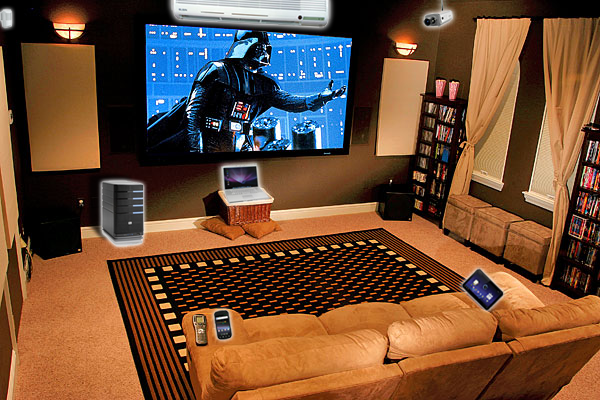
\includegraphics[scale=0.7]{imagens/salaUbiqua}
	\caption{Exemplo de ambiente inteligente.}
	\label{fig:ambienteInteligente}
\end{figure}

Em um ambiente inteligente se faz necessária a adaptabilidade de serviços de forma transparente para os clientes, ou seja, caso um serviço não esteja mais sendo provido por determinado dispositivo, o \emph{smart space} deve identificar esta falha e procurar um outro servidor ~\cite{gomes2007, passarinho2008, paranhos2009}.

\section{DSOA}

Com o objetivo de auxiliar a modelagem de um \emph{smart space} levando em consideração as características de um ambiente ubíquo, foi criada a arquitetura DSOA(\emph{Device Service Oriented Architecture})~\cite{buzetoDSOA2010} que faz uso dos conceitos definidos na SOA(\emph{Service Oriented Architecture}) aplicados a um ambiente inteligente, onde recursos e serviços estarão disponíveis de forma dinâmica. Recursos, segundo a definição na proposta da DSOA, são um grupo de funcionalidades logicamente relacionadas que deverão ser acessíveis por meio de interfaces pré-definidas ~\cite{buzeto2010}. 

Esses recursos serão acessados por meio do \emph{middleware} \emph{uOS}, que utiliza um conjunto de protocolos \emph{uP} (\emph{Ubiquitous Protocols}) como interface de comunicação com \emph{drivers} de recursos disponíveis. A infra-estrutura implementada pelo \emph{uOS} para gerir os recursos do ambiente permite que uma aplicação de um dispositivo acesse recursos, apresentados na forma de um \emph{driver} (\emph{UosDriver}) de outros dispositivos presentes no ambiente.

Quando uma aplicação solicita um serviço de algum recurso, o \emph{uOS} deve tomar uma decisão sobre qual será o dispositivo detentor de tal recurso que provê o serviço solicitado que irá ser escolhido. Para que o \emph{uOS} possa tomar uma decisão inteligente sobre a escolha do dispositivo detentor do recurso, deseja-se que o tipo do recurso seja conhecido. Atualmente, a arquitetura DSOA/\emph{uOS} é pouco maleável nessa definição de tipo de recursos. Os recursos são definidos de forma linear, por exemplo: um recurso de \emph{mouse} com dois botões possui um \emph{driver} associado, já um \emph{mouse} com três botões, possui um outro \emph{driver} associado que não possui nenhuma relação com o primeiro, o que dificulta a tomada de decisão por parte do \emph{middleware}. Existem diversos padrões definidos que fazem uso de uma classificação de dispositivos ou recursos, mas não se adequam à arquitetura DSOA.

O objetivo deste trabalho é definir uma classificação de recursos e a partir desta classificação, prover uma hierarquia de recursos extensível para a arquitetura DSOA do \emph{middleware} de Computação Ubíqua \emph{uOS}. Essa hierarquia irá facilitar a escolha de determinado serviço provido por algum recurso por parte do \emph{uOS} ou de alguma aplicação cliente.


O presente trabalho encontra-se organizado da seguinte maneira: o capítulo 2 fundamenta os conceitos que serão utilizados neste trabalho e apresenta uma visão geral do projeto UbiquitOS, a arquitetura DSOA e o conjunto de protocolos \emph{uP}. O capítulo seguinte descreve a importância da classificação de recursos, bem como as diferentes maneiras de se representa-la. Lista também os principais padrões conhecidos e projetos que utilizam uma classificação para auxilio de suas atividades.
\end{comment}

Este trabalho está organizado da seguinte maneira: O capítulo 2 fundamenta os conceitos que serão utilizados neste trabalho. É iniciado apresentando uma visão geral do projeto UbiquitOS, explicando os principais conceitos da DSOA e mostrando em detalhes os protocolos que constituem o uP. A seção seguinte mostra a importância da classificação de recursos bem como as diferentes maneiras de se classificar e representá-la. Ainda na segunda seção, serão apresentados alguns dos principais padrões conhecidos e projetos de Computação Ubíqua que utilizam uma classificação de recursos ou dispositivos para auxiliar em suas atividades. A seção e o capítulo são finalizados realizando um comparativo entre as diferentes classificações mostradas. No capítulo 3 será apresentada a classificação de recursos proposta por este trabalho. Na primeira seção serão mostrados os tipos básicos definidos pela classificação, o identificador e seus serviços associados. A seção seguinte apresenta o conceito da equivalência de recursos e como é estabelecida uma relação de equivalência entre recursos. O capítulo é concluído detalhando os impactos dessa classificação na arquitetura DSOA/\emph{uOS}. O capítulo 4 é iniciado detalhando como foi realizada a implementação da classificação de recursos no \emph{middleware} \emph{uOS} e termina mostrando o estudo de caso realizado para demonstrar um bom uso da classificação de recursos. No capítulo 5 é apresentada a conclusão deste trabalho e trabalhos que poderão ser realizados a partir da contribuição deste.